% Created by tikzDevice version 0.12 on 2019-03-11 11:52:46
% !TEX encoding = UTF-8 Unicode
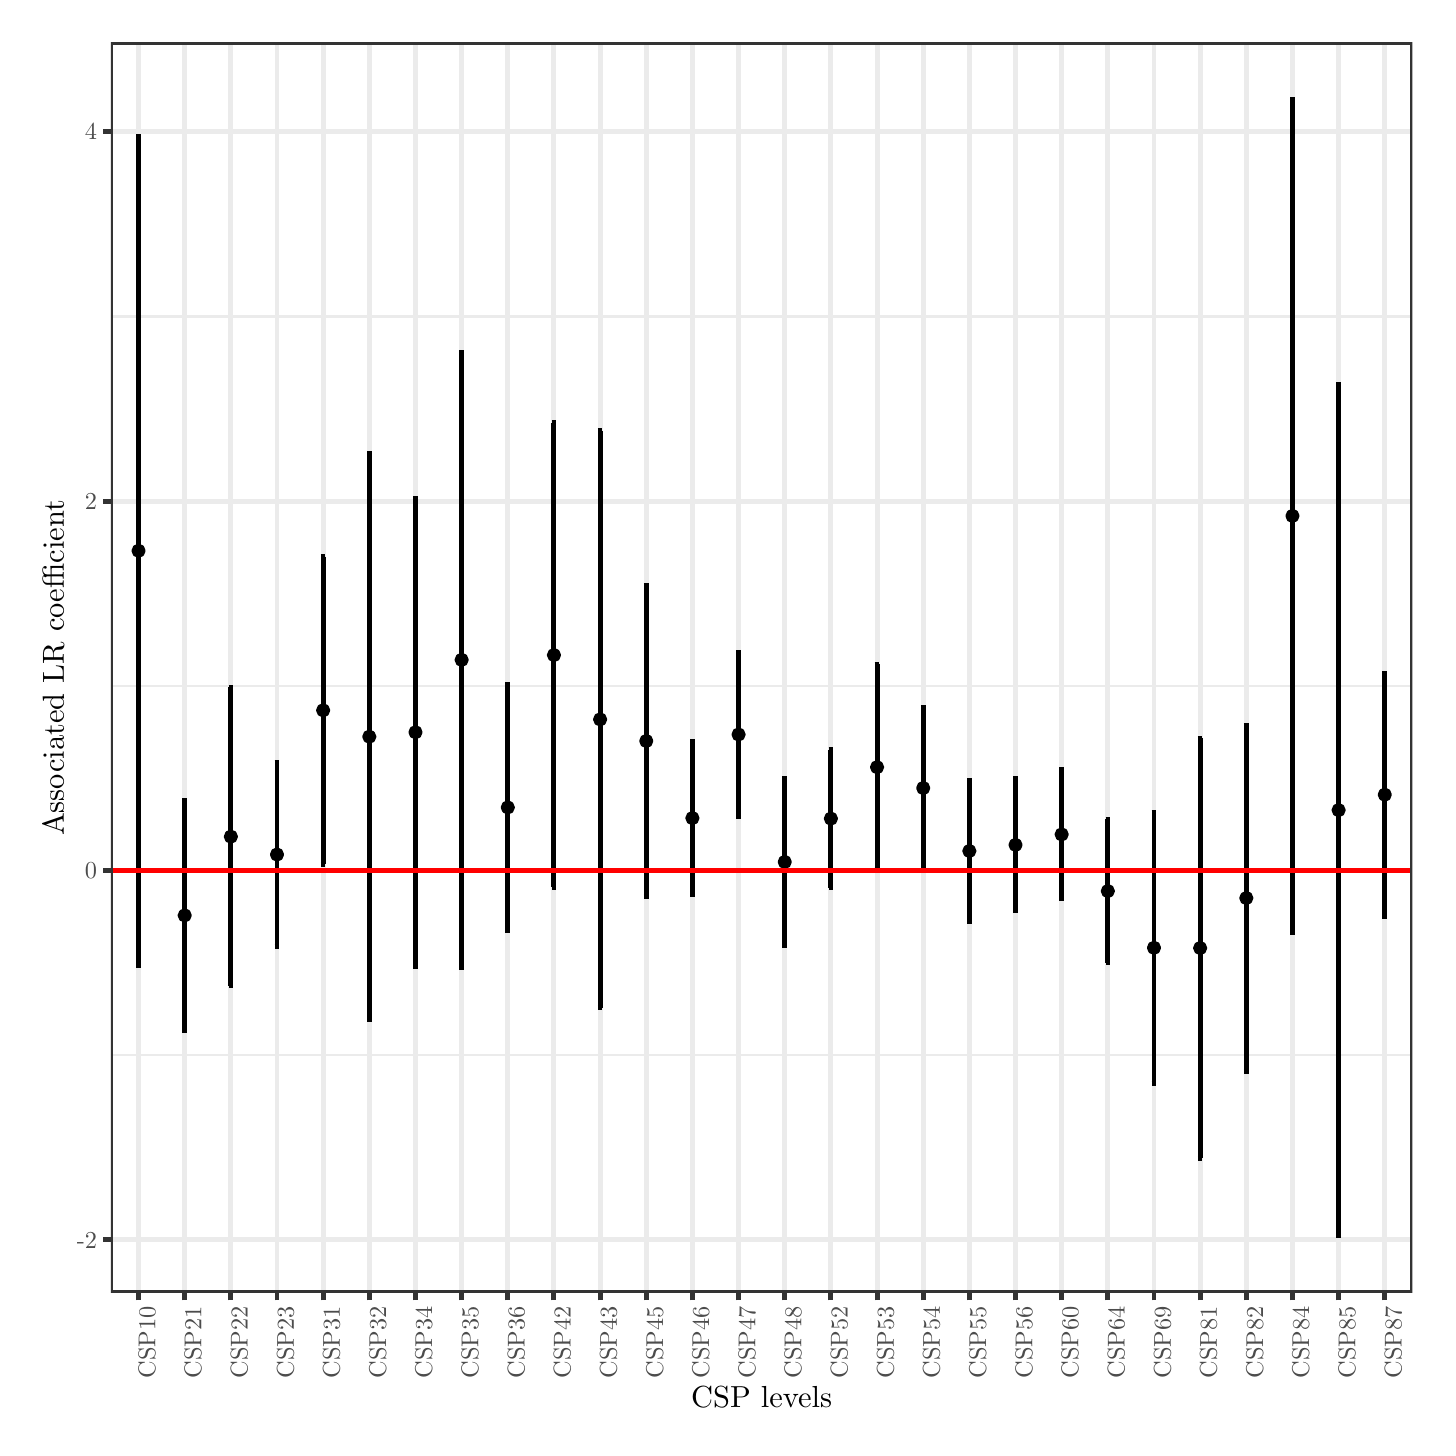
\begin{tikzpicture}[x=1pt,y=1pt]
\definecolor{fillColor}{RGB}{255,255,255}
\path[use as bounding box,fill=fillColor,fill opacity=0.00] (0,0) rectangle (505.89,505.89);
\begin{scope}
\path[clip] (  0.00,  0.00) rectangle (505.89,505.89);
\definecolor{drawColor}{RGB}{255,255,255}
\definecolor{fillColor}{RGB}{255,255,255}

\path[draw=drawColor,line width= 1.8pt,line join=round,line cap=round,fill=fillColor] (  0.00,  0.00) rectangle (505.89,505.89);
\end{scope}
\begin{scope}
\path[clip] ( 30.05, 48.75) rectangle (500.39,500.39);
\definecolor{fillColor}{RGB}{255,255,255}

\path[fill=fillColor] ( 30.05, 48.75) rectangle (500.39,500.39);
\definecolor{drawColor}{gray}{0.92}

\path[draw=drawColor,line width= 0.9pt,line join=round] ( 30.05,134.58) --
	(500.39,134.58);

\path[draw=drawColor,line width= 0.9pt,line join=round] ( 30.05,268.08) --
	(500.39,268.08);

\path[draw=drawColor,line width= 0.9pt,line join=round] ( 30.05,401.59) --
	(500.39,401.59);

\path[draw=drawColor,line width= 1.8pt,line join=round] ( 30.05, 67.82) --
	(500.39, 67.82);

\path[draw=drawColor,line width= 1.8pt,line join=round] ( 30.05,201.33) --
	(500.39,201.33);

\path[draw=drawColor,line width= 1.8pt,line join=round] ( 30.05,334.84) --
	(500.39,334.84);

\path[draw=drawColor,line width= 1.8pt,line join=round] ( 30.05,468.35) --
	(500.39,468.35);

\path[draw=drawColor,line width= 1.8pt,line join=round] ( 40.06, 48.75) --
	( 40.06,500.39);

\path[draw=drawColor,line width= 1.8pt,line join=round] ( 56.74, 48.75) --
	( 56.74,500.39);

\path[draw=drawColor,line width= 1.8pt,line join=round] ( 73.42, 48.75) --
	( 73.42,500.39);

\path[draw=drawColor,line width= 1.8pt,line join=round] ( 90.09, 48.75) --
	( 90.09,500.39);

\path[draw=drawColor,line width= 1.8pt,line join=round] (106.77, 48.75) --
	(106.77,500.39);

\path[draw=drawColor,line width= 1.8pt,line join=round] (123.45, 48.75) --
	(123.45,500.39);

\path[draw=drawColor,line width= 1.8pt,line join=round] (140.13, 48.75) --
	(140.13,500.39);

\path[draw=drawColor,line width= 1.8pt,line join=round] (156.81, 48.75) --
	(156.81,500.39);

\path[draw=drawColor,line width= 1.8pt,line join=round] (173.49, 48.75) --
	(173.49,500.39);

\path[draw=drawColor,line width= 1.8pt,line join=round] (190.17, 48.75) --
	(190.17,500.39);

\path[draw=drawColor,line width= 1.8pt,line join=round] (206.85, 48.75) --
	(206.85,500.39);

\path[draw=drawColor,line width= 1.8pt,line join=round] (223.52, 48.75) --
	(223.52,500.39);

\path[draw=drawColor,line width= 1.8pt,line join=round] (240.20, 48.75) --
	(240.20,500.39);

\path[draw=drawColor,line width= 1.8pt,line join=round] (256.88, 48.75) --
	(256.88,500.39);

\path[draw=drawColor,line width= 1.8pt,line join=round] (273.56, 48.75) --
	(273.56,500.39);

\path[draw=drawColor,line width= 1.8pt,line join=round] (290.24, 48.75) --
	(290.24,500.39);

\path[draw=drawColor,line width= 1.8pt,line join=round] (306.92, 48.75) --
	(306.92,500.39);

\path[draw=drawColor,line width= 1.8pt,line join=round] (323.60, 48.75) --
	(323.60,500.39);

\path[draw=drawColor,line width= 1.8pt,line join=round] (340.27, 48.75) --
	(340.27,500.39);

\path[draw=drawColor,line width= 1.8pt,line join=round] (356.95, 48.75) --
	(356.95,500.39);

\path[draw=drawColor,line width= 1.8pt,line join=round] (373.63, 48.75) --
	(373.63,500.39);

\path[draw=drawColor,line width= 1.8pt,line join=round] (390.31, 48.75) --
	(390.31,500.39);

\path[draw=drawColor,line width= 1.8pt,line join=round] (406.99, 48.75) --
	(406.99,500.39);

\path[draw=drawColor,line width= 1.8pt,line join=round] (423.67, 48.75) --
	(423.67,500.39);

\path[draw=drawColor,line width= 1.8pt,line join=round] (440.35, 48.75) --
	(440.35,500.39);

\path[draw=drawColor,line width= 1.8pt,line join=round] (457.03, 48.75) --
	(457.03,500.39);

\path[draw=drawColor,line width= 1.8pt,line join=round] (473.70, 48.75) --
	(473.70,500.39);

\path[draw=drawColor,line width= 1.8pt,line join=round] (490.38, 48.75) --
	(490.38,500.39);
\definecolor{drawColor}{RGB}{0,0,0}

\path[draw=drawColor,line width= 1.8pt,line join=round] (239.37,247.82) --
	(241.04,247.82);

\path[draw=drawColor,line width= 1.8pt,line join=round] (240.20,247.82) --
	(240.20,192.71);

\path[draw=drawColor,line width= 1.8pt,line join=round] (239.37,192.71) --
	(241.04,192.71);

\path[draw=drawColor,line width= 1.8pt,line join=round] (356.12,234.41) --
	(357.79,234.41);

\path[draw=drawColor,line width= 1.8pt,line join=round] (356.95,234.41) --
	(356.95,186.76);

\path[draw=drawColor,line width= 1.8pt,line join=round] (356.12,186.76) --
	(357.79,186.76);

\path[draw=drawColor,line width= 1.8pt,line join=round] (105.94,314.77) --
	(107.61,314.77);

\path[draw=drawColor,line width= 1.8pt,line join=round] (106.77,314.77) --
	(106.77,203.67);

\path[draw=drawColor,line width= 1.8pt,line join=round] (105.94,203.67) --
	(107.61,203.67);

\path[draw=drawColor,line width= 1.8pt,line join=round] (372.80,237.67) --
	(374.47,237.67);

\path[draw=drawColor,line width= 1.8pt,line join=round] (373.63,237.67) --
	(373.63,191.07);

\path[draw=drawColor,line width= 1.8pt,line join=round] (372.80,191.07) --
	(374.47,191.07);

\path[draw=drawColor,line width= 1.8pt,line join=round] (339.44,233.68) --
	(341.11,233.68);

\path[draw=drawColor,line width= 1.8pt,line join=round] (340.27,233.68) --
	(340.27,183.07);

\path[draw=drawColor,line width= 1.8pt,line join=round] (339.44,183.07) --
	(341.11,183.07);

\path[draw=drawColor,line width= 1.8pt,line join=round] (172.65,268.58) --
	(174.32,268.58);

\path[draw=drawColor,line width= 1.8pt,line join=round] (173.49,268.58) --
	(173.49,179.67);

\path[draw=drawColor,line width= 1.8pt,line join=round] (172.65,179.67) --
	(174.32,179.67);

\path[draw=drawColor,line width= 1.8pt,line join=round] (439.51,253.90) --
	(441.18,253.90);

\path[draw=drawColor,line width= 1.8pt,line join=round] (440.35,253.90) --
	(440.35,128.85);

\path[draw=drawColor,line width= 1.8pt,line join=round] (439.51,128.85) --
	(441.18,128.85);

\path[draw=drawColor,line width= 1.8pt,line join=round] (289.40,245.02) --
	(291.07,245.02);

\path[draw=drawColor,line width= 1.8pt,line join=round] (290.24,245.02) --
	(290.24,195.15);

\path[draw=drawColor,line width= 1.8pt,line join=round] (289.40,195.15) --
	(291.07,195.15);

\path[draw=drawColor,line width= 1.8pt,line join=round] (256.05,280.02) --
	(257.72,280.02);

\path[draw=drawColor,line width= 1.8pt,line join=round] (256.88,280.02) --
	(256.88,220.93);

\path[draw=drawColor,line width= 1.8pt,line join=round] (256.05,220.93) --
	(257.72,220.93);

\path[draw=drawColor,line width= 1.8pt,line join=round] ( 55.90,226.67) --
	( 57.57,226.67);

\path[draw=drawColor,line width= 1.8pt,line join=round] ( 56.74,226.67) --
	( 56.74,143.54);

\path[draw=drawColor,line width= 1.8pt,line join=round] ( 55.90,143.54) --
	( 57.57,143.54);

\path[draw=drawColor,line width= 1.8pt,line join=round] (306.08,275.80) --
	(307.75,275.80);

\path[draw=drawColor,line width= 1.8pt,line join=round] (306.92,275.80) --
	(306.92,201.53);

\path[draw=drawColor,line width= 1.8pt,line join=round] (306.08,201.53) --
	(307.75,201.53);

\path[draw=drawColor,line width= 1.8pt,line join=round] (322.76,260.22) --
	(324.43,260.22);

\path[draw=drawColor,line width= 1.8pt,line join=round] (323.60,260.22) --
	(323.60,202.05);

\path[draw=drawColor,line width= 1.8pt,line join=round] (322.76,202.05) --
	(324.43,202.05);

\path[draw=drawColor,line width= 1.8pt,line join=round] ( 89.26,240.48) --
	( 90.93,240.48);

\path[draw=drawColor,line width= 1.8pt,line join=round] ( 90.09,240.48) --
	( 90.09,173.73);

\path[draw=drawColor,line width= 1.8pt,line join=round] ( 89.26,173.73) --
	( 90.93,173.73);

\path[draw=drawColor,line width= 1.8pt,line join=round] (422.83,249.20) --
	(424.50,249.20);

\path[draw=drawColor,line width= 1.8pt,line join=round] (423.67,249.20) --
	(423.67, 97.43);

\path[draw=drawColor,line width= 1.8pt,line join=round] (422.83, 97.43) --
	(424.50, 97.43);

\path[draw=drawColor,line width= 1.8pt,line join=round] (272.73,234.60) --
	(274.39,234.60);

\path[draw=drawColor,line width= 1.8pt,line join=round] (273.56,234.60) --
	(273.56,174.25);

\path[draw=drawColor,line width= 1.8pt,line join=round] (272.73,174.25) --
	(274.39,174.25);

\path[draw=drawColor,line width= 1.8pt,line join=round] (139.30,335.85) --
	(140.96,335.85);

\path[draw=drawColor,line width= 1.8pt,line join=round] (140.13,335.85) --
	(140.13,166.73);

\path[draw=drawColor,line width= 1.8pt,line join=round] (139.30,166.73) --
	(140.96,166.73);

\path[draw=drawColor,line width= 1.8pt,line join=round] (389.48,219.90) --
	(391.14,219.90);

\path[draw=drawColor,line width= 1.8pt,line join=round] (390.31,219.90) --
	(390.31,167.91);

\path[draw=drawColor,line width= 1.8pt,line join=round] (389.48,167.91) --
	(391.14,167.91);

\path[draw=drawColor,line width= 1.8pt,line join=round] (189.33,363.13) --
	(191.00,363.13);

\path[draw=drawColor,line width= 1.8pt,line join=round] (190.17,363.13) --
	(190.17,195.23);

\path[draw=drawColor,line width= 1.8pt,line join=round] (189.33,195.23) --
	(191.00,195.23);

\path[draw=drawColor,line width= 1.8pt,line join=round] (122.62,352.06) --
	(124.29,352.06);

\path[draw=drawColor,line width= 1.8pt,line join=round] (123.45,352.06) --
	(123.45,147.31);

\path[draw=drawColor,line width= 1.8pt,line join=round] (122.62,147.31) --
	(124.29,147.31);

\path[draw=drawColor,line width= 1.8pt,line join=round] (206.01,360.21) --
	(207.68,360.21);

\path[draw=drawColor,line width= 1.8pt,line join=round] (206.85,360.21) --
	(206.85,151.65);

\path[draw=drawColor,line width= 1.8pt,line join=round] (206.01,151.65) --
	(207.68,151.65);

\path[draw=drawColor,line width= 1.8pt,line join=round] (222.69,304.30) --
	(224.36,304.30);

\path[draw=drawColor,line width= 1.8pt,line join=round] (223.52,304.30) --
	(223.52,191.96);

\path[draw=drawColor,line width= 1.8pt,line join=round] (222.69,191.96) --
	(224.36,191.96);

\path[draw=drawColor,line width= 1.8pt,line join=round] (406.16,222.39) --
	(407.82,222.39);

\path[draw=drawColor,line width= 1.8pt,line join=round] (406.99,222.39) --
	(406.99,124.41);

\path[draw=drawColor,line width= 1.8pt,line join=round] (406.16,124.41) --
	(407.82,124.41);

\path[draw=drawColor,line width= 1.8pt,line join=round] ( 72.58,267.52) --
	( 74.25,267.52);

\path[draw=drawColor,line width= 1.8pt,line join=round] ( 73.42,267.52) --
	( 73.42,159.62);

\path[draw=drawColor,line width= 1.8pt,line join=round] ( 72.58,159.62) --
	( 74.25,159.62);

\path[draw=drawColor,line width= 1.8pt,line join=round] (155.98,388.62) --
	(157.64,388.62);

\path[draw=drawColor,line width= 1.8pt,line join=round] (156.81,388.62) --
	(156.81,166.28);

\path[draw=drawColor,line width= 1.8pt,line join=round] (155.98,166.28) --
	(157.64,166.28);

\path[draw=drawColor,line width= 1.8pt,line join=round] (456.19,479.86) --
	(457.86,479.86);

\path[draw=drawColor,line width= 1.8pt,line join=round] (457.03,479.86) --
	(457.03,179.07);

\path[draw=drawColor,line width= 1.8pt,line join=round] (456.19,179.07) --
	(457.86,179.07);

\path[draw=drawColor,line width= 1.8pt,line join=round] ( 39.22,466.63) --
	( 40.89,466.63);

\path[draw=drawColor,line width= 1.8pt,line join=round] ( 40.06,466.63) --
	( 40.06,167.09);

\path[draw=drawColor,line width= 1.8pt,line join=round] ( 39.22,167.09) --
	( 40.89,167.09);

\path[draw=drawColor,line width= 1.8pt,line join=round] (489.55,272.67) --
	(491.22,272.67);

\path[draw=drawColor,line width= 1.8pt,line join=round] (490.38,272.67) --
	(490.38,184.79);

\path[draw=drawColor,line width= 1.8pt,line join=round] (489.55,184.79) --
	(491.22,184.79);

\path[draw=drawColor,line width= 1.8pt,line join=round] (472.87,377.02) --
	(474.54,377.02);

\path[draw=drawColor,line width= 1.8pt,line join=round] (473.70,377.02) --
	(473.70, 69.28);

\path[draw=drawColor,line width= 1.8pt,line join=round] (472.87, 69.28) --
	(474.54, 69.28);
\definecolor{fillColor}{RGB}{0,0,0}

\path[draw=drawColor,line width= 1.2pt,line join=round,line cap=round,fill=fillColor] (240.20,220.27) circle (  1.96);

\path[draw=drawColor,line width= 1.2pt,line join=round,line cap=round,fill=fillColor] (356.95,210.59) circle (  1.96);

\path[draw=drawColor,line width= 1.2pt,line join=round,line cap=round,fill=fillColor] (106.77,259.22) circle (  1.96);

\path[draw=drawColor,line width= 1.2pt,line join=round,line cap=round,fill=fillColor] (373.63,214.37) circle (  1.96);

\path[draw=drawColor,line width= 1.2pt,line join=round,line cap=round,fill=fillColor] (340.27,208.38) circle (  1.96);

\path[draw=drawColor,line width= 1.2pt,line join=round,line cap=round,fill=fillColor] (173.49,224.12) circle (  1.96);

\path[draw=drawColor,line width= 1.2pt,line join=round,line cap=round,fill=fillColor] (440.35,191.38) circle (  1.96);

\path[draw=drawColor,line width= 1.2pt,line join=round,line cap=round,fill=fillColor] (290.24,220.09) circle (  1.96);

\path[draw=drawColor,line width= 1.2pt,line join=round,line cap=round,fill=fillColor] (256.88,250.48) circle (  1.96);

\path[draw=drawColor,line width= 1.2pt,line join=round,line cap=round,fill=fillColor] ( 56.74,185.11) circle (  1.96);

\path[draw=drawColor,line width= 1.2pt,line join=round,line cap=round,fill=fillColor] (306.92,238.67) circle (  1.96);

\path[draw=drawColor,line width= 1.2pt,line join=round,line cap=round,fill=fillColor] (323.60,231.13) circle (  1.96);

\path[draw=drawColor,line width= 1.2pt,line join=round,line cap=round,fill=fillColor] ( 90.09,207.10) circle (  1.96);

\path[draw=drawColor,line width= 1.2pt,line join=round,line cap=round,fill=fillColor] (423.67,173.32) circle (  1.96);

\path[draw=drawColor,line width= 1.2pt,line join=round,line cap=round,fill=fillColor] (273.56,204.43) circle (  1.96);

\path[draw=drawColor,line width= 1.2pt,line join=round,line cap=round,fill=fillColor] (140.13,251.29) circle (  1.96);

\path[draw=drawColor,line width= 1.2pt,line join=round,line cap=round,fill=fillColor] (390.31,193.90) circle (  1.96);

\path[draw=drawColor,line width= 1.2pt,line join=round,line cap=round,fill=fillColor] (190.17,279.18) circle (  1.96);

\path[draw=drawColor,line width= 1.2pt,line join=round,line cap=round,fill=fillColor] (123.45,249.69) circle (  1.96);

\path[draw=drawColor,line width= 1.2pt,line join=round,line cap=round,fill=fillColor] (206.85,255.93) circle (  1.96);

\path[draw=drawColor,line width= 1.2pt,line join=round,line cap=round,fill=fillColor] (223.52,248.13) circle (  1.96);

\path[draw=drawColor,line width= 1.2pt,line join=round,line cap=round,fill=fillColor] (406.99,173.40) circle (  1.96);

\path[draw=drawColor,line width= 1.2pt,line join=round,line cap=round,fill=fillColor] ( 73.42,213.57) circle (  1.96);

\path[draw=drawColor,line width= 1.2pt,line join=round,line cap=round,fill=fillColor] (156.81,277.45) circle (  1.96);

\path[draw=drawColor,line width= 1.2pt,line join=round,line cap=round,fill=fillColor] (457.03,329.46) circle (  1.96);

\path[draw=drawColor,line width= 1.2pt,line join=round,line cap=round,fill=fillColor] ( 40.06,316.86) circle (  1.96);

\path[draw=drawColor,line width= 1.2pt,line join=round,line cap=round,fill=fillColor] (490.38,228.73) circle (  1.96);

\path[draw=drawColor,line width= 1.2pt,line join=round,line cap=round,fill=fillColor] (473.70,223.15) circle (  1.96);
\definecolor{drawColor}{RGB}{255,0,0}

\path[draw=drawColor,line width= 1.8pt,line join=round] ( 30.05,201.33) -- (500.39,201.33);
\definecolor{drawColor}{gray}{0.20}

\path[draw=drawColor,line width= 1.8pt,line join=round,line cap=round] ( 30.05, 48.75) rectangle (500.39,500.39);
\end{scope}
\begin{scope}
\path[clip] (  0.00,  0.00) rectangle (505.89,505.89);
\definecolor{drawColor}{gray}{0.30}

\node[text=drawColor,anchor=base east,inner sep=0pt, outer sep=0pt, scale=  0.88] at ( 25.10, 64.79) {-2};

\node[text=drawColor,anchor=base east,inner sep=0pt, outer sep=0pt, scale=  0.88] at ( 25.10,198.30) {0};

\node[text=drawColor,anchor=base east,inner sep=0pt, outer sep=0pt, scale=  0.88] at ( 25.10,331.81) {2};

\node[text=drawColor,anchor=base east,inner sep=0pt, outer sep=0pt, scale=  0.88] at ( 25.10,465.32) {4};
\end{scope}
\begin{scope}
\path[clip] (  0.00,  0.00) rectangle (505.89,505.89);
\definecolor{drawColor}{gray}{0.20}

\path[draw=drawColor,line width= 1.8pt,line join=round] ( 27.30, 67.82) --
	( 30.05, 67.82);

\path[draw=drawColor,line width= 1.8pt,line join=round] ( 27.30,201.33) --
	( 30.05,201.33);

\path[draw=drawColor,line width= 1.8pt,line join=round] ( 27.30,334.84) --
	( 30.05,334.84);

\path[draw=drawColor,line width= 1.8pt,line join=round] ( 27.30,468.35) --
	( 30.05,468.35);
\end{scope}
\begin{scope}
\path[clip] (  0.00,  0.00) rectangle (505.89,505.89);
\definecolor{drawColor}{gray}{0.20}

\path[draw=drawColor,line width= 1.8pt,line join=round] ( 40.06, 46.00) --
	( 40.06, 48.75);

\path[draw=drawColor,line width= 1.8pt,line join=round] ( 56.74, 46.00) --
	( 56.74, 48.75);

\path[draw=drawColor,line width= 1.8pt,line join=round] ( 73.42, 46.00) --
	( 73.42, 48.75);

\path[draw=drawColor,line width= 1.8pt,line join=round] ( 90.09, 46.00) --
	( 90.09, 48.75);

\path[draw=drawColor,line width= 1.8pt,line join=round] (106.77, 46.00) --
	(106.77, 48.75);

\path[draw=drawColor,line width= 1.8pt,line join=round] (123.45, 46.00) --
	(123.45, 48.75);

\path[draw=drawColor,line width= 1.8pt,line join=round] (140.13, 46.00) --
	(140.13, 48.75);

\path[draw=drawColor,line width= 1.8pt,line join=round] (156.81, 46.00) --
	(156.81, 48.75);

\path[draw=drawColor,line width= 1.8pt,line join=round] (173.49, 46.00) --
	(173.49, 48.75);

\path[draw=drawColor,line width= 1.8pt,line join=round] (190.17, 46.00) --
	(190.17, 48.75);

\path[draw=drawColor,line width= 1.8pt,line join=round] (206.85, 46.00) --
	(206.85, 48.75);

\path[draw=drawColor,line width= 1.8pt,line join=round] (223.52, 46.00) --
	(223.52, 48.75);

\path[draw=drawColor,line width= 1.8pt,line join=round] (240.20, 46.00) --
	(240.20, 48.75);

\path[draw=drawColor,line width= 1.8pt,line join=round] (256.88, 46.00) --
	(256.88, 48.75);

\path[draw=drawColor,line width= 1.8pt,line join=round] (273.56, 46.00) --
	(273.56, 48.75);

\path[draw=drawColor,line width= 1.8pt,line join=round] (290.24, 46.00) --
	(290.24, 48.75);

\path[draw=drawColor,line width= 1.8pt,line join=round] (306.92, 46.00) --
	(306.92, 48.75);

\path[draw=drawColor,line width= 1.8pt,line join=round] (323.60, 46.00) --
	(323.60, 48.75);

\path[draw=drawColor,line width= 1.8pt,line join=round] (340.27, 46.00) --
	(340.27, 48.75);

\path[draw=drawColor,line width= 1.8pt,line join=round] (356.95, 46.00) --
	(356.95, 48.75);

\path[draw=drawColor,line width= 1.8pt,line join=round] (373.63, 46.00) --
	(373.63, 48.75);

\path[draw=drawColor,line width= 1.8pt,line join=round] (390.31, 46.00) --
	(390.31, 48.75);

\path[draw=drawColor,line width= 1.8pt,line join=round] (406.99, 46.00) --
	(406.99, 48.75);

\path[draw=drawColor,line width= 1.8pt,line join=round] (423.67, 46.00) --
	(423.67, 48.75);

\path[draw=drawColor,line width= 1.8pt,line join=round] (440.35, 46.00) --
	(440.35, 48.75);

\path[draw=drawColor,line width= 1.8pt,line join=round] (457.03, 46.00) --
	(457.03, 48.75);

\path[draw=drawColor,line width= 1.8pt,line join=round] (473.70, 46.00) --
	(473.70, 48.75);

\path[draw=drawColor,line width= 1.8pt,line join=round] (490.38, 46.00) --
	(490.38, 48.75);
\end{scope}
\begin{scope}
\path[clip] (  0.00,  0.00) rectangle (505.89,505.89);
\definecolor{drawColor}{gray}{0.30}

\node[text=drawColor,rotate= 90.00,anchor=base east,inner sep=0pt, outer sep=0pt, scale=  0.88] at ( 46.12, 43.80) {CSP10};

\node[text=drawColor,rotate= 90.00,anchor=base east,inner sep=0pt, outer sep=0pt, scale=  0.88] at ( 62.80, 43.80) {CSP21};

\node[text=drawColor,rotate= 90.00,anchor=base east,inner sep=0pt, outer sep=0pt, scale=  0.88] at ( 79.48, 43.80) {CSP22};

\node[text=drawColor,rotate= 90.00,anchor=base east,inner sep=0pt, outer sep=0pt, scale=  0.88] at ( 96.16, 43.80) {CSP23};

\node[text=drawColor,rotate= 90.00,anchor=base east,inner sep=0pt, outer sep=0pt, scale=  0.88] at (112.83, 43.80) {CSP31};

\node[text=drawColor,rotate= 90.00,anchor=base east,inner sep=0pt, outer sep=0pt, scale=  0.88] at (129.51, 43.80) {CSP32};

\node[text=drawColor,rotate= 90.00,anchor=base east,inner sep=0pt, outer sep=0pt, scale=  0.88] at (146.19, 43.80) {CSP34};

\node[text=drawColor,rotate= 90.00,anchor=base east,inner sep=0pt, outer sep=0pt, scale=  0.88] at (162.87, 43.80) {CSP35};

\node[text=drawColor,rotate= 90.00,anchor=base east,inner sep=0pt, outer sep=0pt, scale=  0.88] at (179.55, 43.80) {CSP36};

\node[text=drawColor,rotate= 90.00,anchor=base east,inner sep=0pt, outer sep=0pt, scale=  0.88] at (196.23, 43.80) {CSP42};

\node[text=drawColor,rotate= 90.00,anchor=base east,inner sep=0pt, outer sep=0pt, scale=  0.88] at (212.91, 43.80) {CSP43};

\node[text=drawColor,rotate= 90.00,anchor=base east,inner sep=0pt, outer sep=0pt, scale=  0.88] at (229.58, 43.80) {CSP45};

\node[text=drawColor,rotate= 90.00,anchor=base east,inner sep=0pt, outer sep=0pt, scale=  0.88] at (246.26, 43.80) {CSP46};

\node[text=drawColor,rotate= 90.00,anchor=base east,inner sep=0pt, outer sep=0pt, scale=  0.88] at (262.94, 43.80) {CSP47};

\node[text=drawColor,rotate= 90.00,anchor=base east,inner sep=0pt, outer sep=0pt, scale=  0.88] at (279.62, 43.80) {CSP48};

\node[text=drawColor,rotate= 90.00,anchor=base east,inner sep=0pt, outer sep=0pt, scale=  0.88] at (296.30, 43.80) {CSP52};

\node[text=drawColor,rotate= 90.00,anchor=base east,inner sep=0pt, outer sep=0pt, scale=  0.88] at (312.98, 43.80) {CSP53};

\node[text=drawColor,rotate= 90.00,anchor=base east,inner sep=0pt, outer sep=0pt, scale=  0.88] at (329.66, 43.80) {CSP54};

\node[text=drawColor,rotate= 90.00,anchor=base east,inner sep=0pt, outer sep=0pt, scale=  0.88] at (346.34, 43.80) {CSP55};

\node[text=drawColor,rotate= 90.00,anchor=base east,inner sep=0pt, outer sep=0pt, scale=  0.88] at (363.01, 43.80) {CSP56};

\node[text=drawColor,rotate= 90.00,anchor=base east,inner sep=0pt, outer sep=0pt, scale=  0.88] at (379.69, 43.80) {CSP60};

\node[text=drawColor,rotate= 90.00,anchor=base east,inner sep=0pt, outer sep=0pt, scale=  0.88] at (396.37, 43.80) {CSP64};

\node[text=drawColor,rotate= 90.00,anchor=base east,inner sep=0pt, outer sep=0pt, scale=  0.88] at (413.05, 43.80) {CSP69};

\node[text=drawColor,rotate= 90.00,anchor=base east,inner sep=0pt, outer sep=0pt, scale=  0.88] at (429.73, 43.80) {CSP81};

\node[text=drawColor,rotate= 90.00,anchor=base east,inner sep=0pt, outer sep=0pt, scale=  0.88] at (446.41, 43.80) {CSP82};

\node[text=drawColor,rotate= 90.00,anchor=base east,inner sep=0pt, outer sep=0pt, scale=  0.88] at (463.09, 43.80) {CSP84};

\node[text=drawColor,rotate= 90.00,anchor=base east,inner sep=0pt, outer sep=0pt, scale=  0.88] at (479.76, 43.80) {CSP85};

\node[text=drawColor,rotate= 90.00,anchor=base east,inner sep=0pt, outer sep=0pt, scale=  0.88] at (496.44, 43.80) {CSP87};
\end{scope}
\begin{scope}
\path[clip] (  0.00,  0.00) rectangle (505.89,505.89);
\definecolor{drawColor}{RGB}{0,0,0}

\node[text=drawColor,anchor=base,inner sep=0pt, outer sep=0pt, scale=  1.10] at (265.22,  7.44) {CSP levels};
\end{scope}
\begin{scope}
\path[clip] (  0.00,  0.00) rectangle (505.89,505.89);
\definecolor{drawColor}{RGB}{0,0,0}

\node[text=drawColor,rotate= 90.00,anchor=base,inner sep=0pt, outer sep=0pt, scale=  1.10] at ( 13.08,274.57) {Associated LR coefficient};
\end{scope}
\end{tikzpicture}
